

\tikzset{every picture/.style={line width=0.75pt}} %set default line width to 0.75pt        

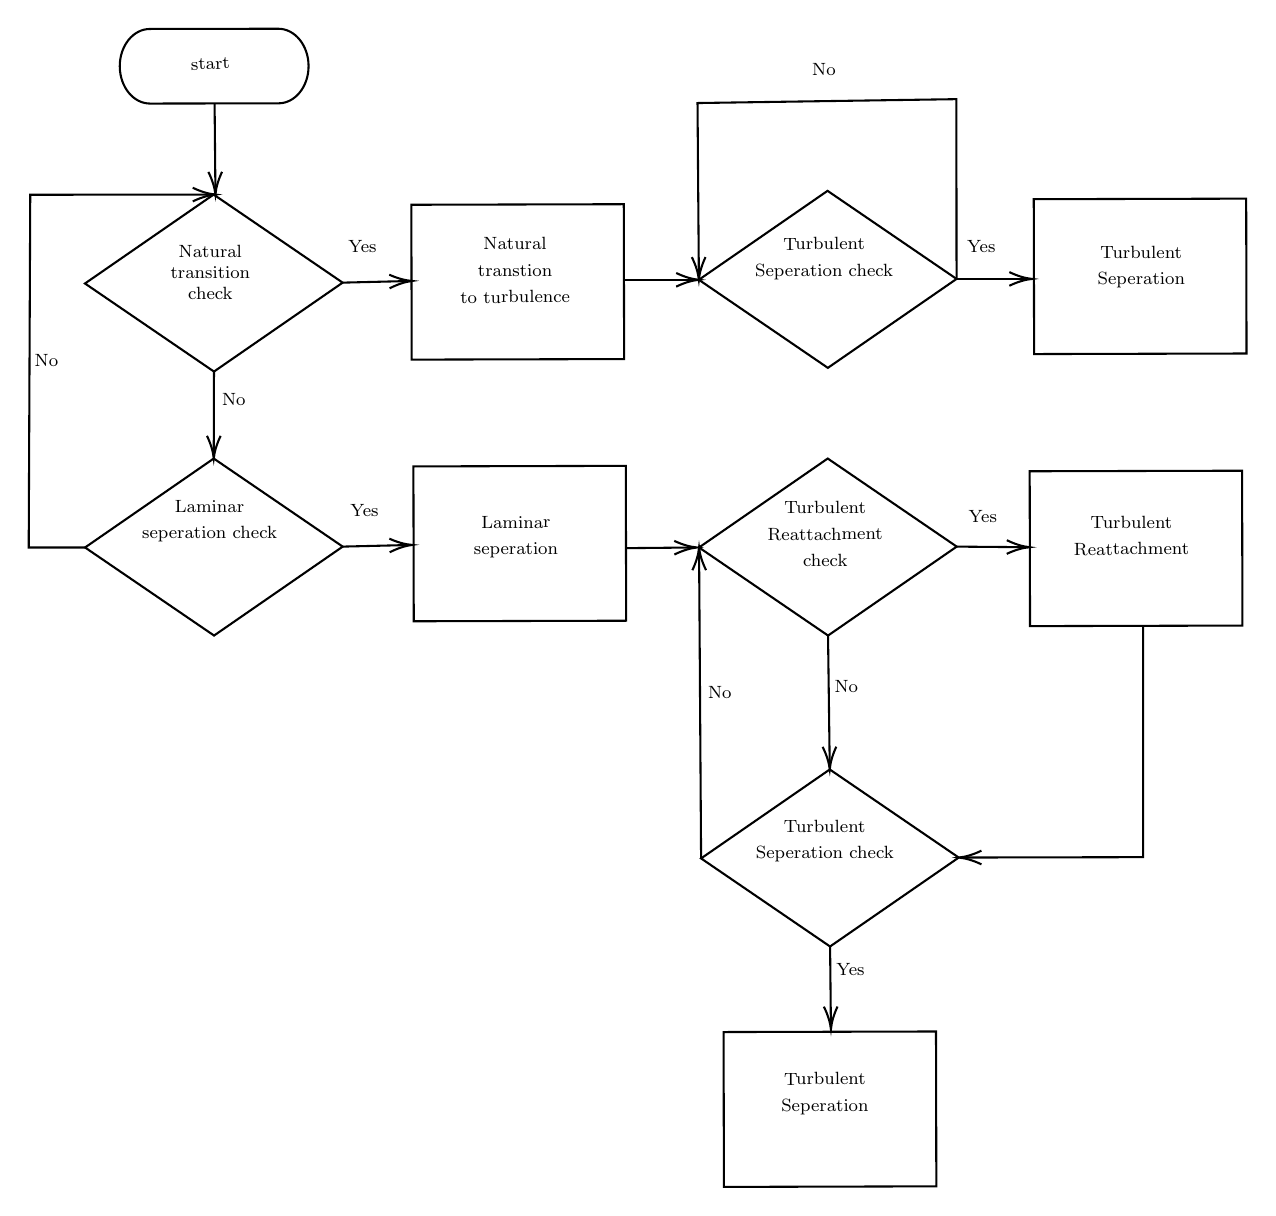
\begin{tikzpicture}[x=0.75pt,y=0.75pt,yscale=-1,xscale=1]
%uncomment if require: \path (0,734); %set diagram left start at 0, and has height of 734

%Flowchart: Terminator [id:dp7207071910268746] 
\draw   (67.63,154.62) -- (129.49,154.51) .. controls (137.52,154.5) and (144.06,162.53) .. (144.09,172.46) .. controls (144.12,182.38) and (137.62,190.44) .. (129.59,190.45) -- (67.73,190.56) .. controls (59.7,190.57) and (53.16,182.54) .. (53.13,172.61) .. controls (53.1,162.69) and (59.6,154.63) .. (67.63,154.62) -- cycle ;
%Straight Lines [id:da10986730772092312] 
\draw    (98.82,190.8) -- (99.21,232.4) ;
\draw [shift={(99.22,234.4)}, rotate = 269.47] [color={rgb, 255:red, 0; green, 0; blue, 0 }  ][line width=0.75]    (10.93,-3.29) .. controls (6.95,-1.4) and (3.31,-0.3) .. (0,0) .. controls (3.31,0.3) and (6.95,1.4) .. (10.93,3.29)   ;
%Straight Lines [id:da11218528639690684] 
\draw    (98.52,319.7) -- (98.41,359.58) ;
\draw [shift={(98.41,361.58)}, rotate = 270.15] [color={rgb, 255:red, 0; green, 0; blue, 0 }  ][line width=0.75]    (10.93,-3.29) .. controls (6.95,-1.4) and (3.31,-0.3) .. (0,0) .. controls (3.31,0.3) and (6.95,1.4) .. (10.93,3.29)   ;
%Flowchart: Decision [id:dp47636663676641755] 
\draw   (98.41,361.58) -- (160.55,404.02) -- (98.56,446.87) -- (36.41,404.44) -- cycle ;
%Flowchart: Process [id:dp0035186106511891913] 
\draw   (193.61,239.32) -- (295.96,239.05) -- (296.13,313.66) -- (193.78,313.93) -- cycle ;
%Straight Lines [id:da41405154544556755] 
\draw    (160.52,276.84) -- (191.97,276.07) ;
\draw [shift={(193.97,276.03)}, rotate = 538.61] [color={rgb, 255:red, 0; green, 0; blue, 0 }  ][line width=0.75]    (10.93,-3.29) .. controls (6.95,-1.4) and (3.31,-0.3) .. (0,0) .. controls (3.31,0.3) and (6.95,1.4) .. (10.93,3.29)   ;
%Straight Lines [id:da4839414628019604] 
\draw    (36.41,404.44) -- (9.26,404.43) -- (10,234.5) -- (97.22,234.4) ;
\draw [shift={(99.22,234.4)}, rotate = 539.94] [color={rgb, 255:red, 0; green, 0; blue, 0 }  ][line width=0.75]    (10.93,-3.29) .. controls (6.95,-1.4) and (3.31,-0.3) .. (0,0) .. controls (3.31,0.3) and (6.95,1.4) .. (10.93,3.29)   ;
%Straight Lines [id:da47695648438676885] 
\draw    (295.76,275.47) -- (330.14,275.47) ;
\draw [shift={(332.14,275.47)}, rotate = 180] [color={rgb, 255:red, 0; green, 0; blue, 0 }  ][line width=0.75]    (10.93,-3.29) .. controls (6.95,-1.4) and (3.31,-0.3) .. (0,0) .. controls (3.31,0.3) and (6.95,1.4) .. (10.93,3.29)   ;
%Flowchart: Decision [id:dp5291766920258706] 
\draw   (98.37,234.4) -- (160.52,276.84) -- (98.52,319.69) -- (36.37,277.25) -- cycle ;
%Flowchart: Process [id:dp6243738863575946] 
\draw   (194.6,365.38) -- (296.94,365.11) -- (297.11,439.72) -- (194.77,439.99) -- cycle ;

%Flowchart: Process [id:dp6109994002876044] 
\draw   (493.49,236.64) -- (595.83,236.37) -- (596,310.98) -- (493.66,311.25) -- cycle ;
%Flowchart: Decision [id:dp19310726941760736] 
\draw   (394.14,232.61) -- (456.29,275.05) -- (394.29,317.9) -- (332.14,275.46) -- cycle ;
%Flowchart: Decision [id:dp374284511592351] 
\draw   (395.21,511.39) -- (457.35,553.83) -- (395.35,596.68) -- (333.21,554.24) -- cycle ;
%Flowchart: Decision [id:dp9780902027233841] 
\draw   (394.22,361.58) -- (456.37,404.02) -- (394.37,446.87) -- (332.22,404.44) -- cycle ;
%Straight Lines [id:da6310642789542652] 
\draw    (160.55,404.02) -- (192.01,403.26) ;
\draw [shift={(194.01,403.21)}, rotate = 538.61] [color={rgb, 255:red, 0; green, 0; blue, 0 }  ][line width=0.75]    (10.93,-3.29) .. controls (6.95,-1.4) and (3.31,-0.3) .. (0,0) .. controls (3.31,0.3) and (6.95,1.4) .. (10.93,3.29)   ;
%Straight Lines [id:da12370255545736619] 
\draw    (456.29,275.05) -- (490.66,275.05) ;
\draw [shift={(492.66,275.05)}, rotate = 180] [color={rgb, 255:red, 0; green, 0; blue, 0 }  ][line width=0.75]    (10.93,-3.29) .. controls (6.95,-1.4) and (3.31,-0.3) .. (0,0) .. controls (3.31,0.3) and (6.95,1.4) .. (10.93,3.29)   ;
%Straight Lines [id:da6933448349630812] 
\draw    (297.08,404.76) -- (329.24,404.45) ;
\draw [shift={(331.24,404.44)}, rotate = 539.46] [color={rgb, 255:red, 0; green, 0; blue, 0 }  ][line width=0.75]    (10.93,-3.29) .. controls (6.95,-1.4) and (3.31,-0.3) .. (0,0) .. controls (3.31,0.3) and (6.95,1.4) .. (10.93,3.29)   ;
%Straight Lines [id:da4268759513220136] 
\draw    (456.29,275.05) -- (456.2,188.44) -- (331.49,190.31) -- (332.13,273.47) ;
\draw [shift={(332.14,275.47)}, rotate = 269.56] [color={rgb, 255:red, 0; green, 0; blue, 0 }  ][line width=0.75]    (10.93,-3.29) .. controls (6.95,-1.4) and (3.31,-0.3) .. (0,0) .. controls (3.31,0.3) and (6.95,1.4) .. (10.93,3.29)   ;
%Straight Lines [id:da994392836584868] 
\draw    (394.37,446.87) -- (395.18,509.39) ;
\draw [shift={(395.2,511.39)}, rotate = 269.26] [color={rgb, 255:red, 0; green, 0; blue, 0 }  ][line width=0.75]    (10.93,-3.29) .. controls (6.95,-1.4) and (3.31,-0.3) .. (0,0) .. controls (3.31,0.3) and (6.95,1.4) .. (10.93,3.29)   ;
%Straight Lines [id:da857618285731965] 
\draw    (456.37,404.02) -- (489.42,404.3) ;
\draw [shift={(491.42,404.31)}, rotate = 180.47] [color={rgb, 255:red, 0; green, 0; blue, 0 }  ][line width=0.75]    (10.93,-3.29) .. controls (6.95,-1.4) and (3.31,-0.3) .. (0,0) .. controls (3.31,0.3) and (6.95,1.4) .. (10.93,3.29)   ;
%Straight Lines [id:da4592324807700441] 
\draw    (395.36,596.68) -- (395.75,634.57) ;
\draw [shift={(395.77,636.57)}, rotate = 269.4] [color={rgb, 255:red, 0; green, 0; blue, 0 }  ][line width=0.75]    (10.93,-3.29) .. controls (6.95,-1.4) and (3.31,-0.3) .. (0,0) .. controls (3.31,0.3) and (6.95,1.4) .. (10.93,3.29)   ;
%Flowchart: Process [id:dp46735660020681147] 
\draw   (344.04,637.9) -- (446.39,637.63) -- (446.55,712.24) -- (344.21,712.51) -- cycle ;
%Flowchart: Process [id:dp5152442854440118] 
\draw   (491.52,367.72) -- (593.86,367.45) -- (594.03,442.06) -- (491.69,442.33) -- cycle ;
%Straight Lines [id:da7889844522327492] 
\draw    (333.21,554.24) -- (332.24,406.44) ;
\draw [shift={(332.23,404.44)}, rotate = 449.62] [color={rgb, 255:red, 0; green, 0; blue, 0 }  ][line width=0.75]    (10.93,-3.29) .. controls (6.95,-1.4) and (3.31,-0.3) .. (0,0) .. controls (3.31,0.3) and (6.95,1.4) .. (10.93,3.29)   ;
%Straight Lines [id:da7830600664422521] 
\draw    (546.2,442.63) -- (546.2,553.64) -- (459.35,553.82) ;
\draw [shift={(457.35,553.83)}, rotate = 359.88] [color={rgb, 255:red, 0; green, 0; blue, 0 }  ][line width=0.75]    (10.93,-3.29) .. controls (6.95,-1.4) and (3.31,-0.3) .. (0,0) .. controls (3.31,0.3) and (6.95,1.4) .. (10.93,3.29)   ;

% Text Node
\draw (162.01,255.44) node [anchor=north west][inner sep=0.75pt]  [rotate=-359.86,xscale=0.8,yscale=0.8] [align=left] {{\footnotesize Yes}};
% Text Node
\draw (101.21,329.24) node [anchor=north west][inner sep=0.75pt]  [rotate=-359.86,xscale=0.8,yscale=0.8] [align=left] {{\footnotesize No}};
% Text Node
\draw (460.19,255.43) node [anchor=north west][inner sep=0.75pt]  [rotate=-359.86,xscale=0.8,yscale=0.8] [align=left] {{\footnotesize Yes}};
% Text Node
\draw (10.92,310.42) node [anchor=north west][inner sep=0.75pt]  [rotate=-359.86,xscale=0.8,yscale=0.8] [align=left] {{\footnotesize No}};
% Text Node
\draw (356.18,254.04) node [anchor=north west][inner sep=0.75pt]  [rotate=-359.86,xscale=0.8,yscale=0.8] [align=left] {\begin{minipage}[lt]{65.779375pt}\setlength\topsep{0pt}
\begin{center}
{\footnotesize Turbulent \ }\\{\footnotesize Seperation check}
\end{center}

\end{minipage}};
% Text Node
\draw (86.09,168.01) node [anchor=north west][inner sep=0.75pt]  [font=\footnotesize,rotate=-358.05,xscale=0.8,yscale=0.8] [align=left] {{\footnotesize start}};
% Text Node
\draw (60,257.54) node [anchor=north west][inner sep=0.75pt]  [font=\footnotesize,rotate=-359.86,xscale=0.8,yscale=0.8] [align=left] {\begin{minipage}[lt]{66.671875pt}\setlength\topsep{0pt}
\begin{center}
{\footnotesize Natural transition }\\{\footnotesize check}
\end{center}

\end{minipage}};
% Text Node
\draw (60.8,380.5) node [anchor=north west][inner sep=0.75pt]  [rotate=-359.86,xscale=0.8,yscale=0.8] [align=left] {\begin{minipage}[lt]{64.419375pt}\setlength\topsep{0pt}
\begin{center}
{\footnotesize Laminar}\\{\footnotesize seperation check}
\end{center}

\end{minipage}};
% Text Node
\draw (209,253.99) node [anchor=north west][inner sep=0.75pt]  [rotate=-359.86,xscale=0.8,yscale=0.8] [align=left] {\begin{minipage}[lt]{62.591875pt}\setlength\topsep{0pt}
\begin{center}
{\footnotesize Natural transtion}\\{\footnotesize  to turbulence}
\end{center}

\end{minipage}};
% Text Node
\draw (221,388.11) node [anchor=north west][inner sep=0.75pt]  [rotate=-359.86,xscale=0.8,yscale=0.8] [align=left] {\begin{minipage}[lt]{40.831875000000004pt}\setlength\topsep{0pt}
\begin{center}
{\footnotesize Laminar }\\{\footnotesize seperation}
\end{center}

\end{minipage}};
% Text Node
\draw (162.99,382.51) node [anchor=north west][inner sep=0.75pt]  [rotate=-359.86,xscale=0.8,yscale=0.8] [align=left] {{\footnotesize Yes}};
% Text Node
\draw (521.57,258.06) node [anchor=north west][inner sep=0.75pt]  [rotate=-359.86,xscale=0.8,yscale=0.8] [align=left] {\begin{minipage}[lt]{42.191875pt}\setlength\topsep{0pt}
\begin{center}
{\footnotesize Turbulent \ }\\{\footnotesize Seperation}
\end{center}

\end{minipage}};
% Text Node
\draw (362,381) node [anchor=north west][inner sep=0.75pt]  [rotate=-359.86,xscale=0.8,yscale=0.8] [align=left] {\begin{minipage}[lt]{55.791875000000005pt}\setlength\topsep{0pt}
\begin{center}
{\footnotesize Turbulent \ }\\{\footnotesize Reattachment }\\{\footnotesize check}
\end{center}

\end{minipage}};
% Text Node
\draw (385.51,170.09) node [anchor=north west][inner sep=0.75pt]  [rotate=-359.86,xscale=0.8,yscale=0.8] [align=left] {{\footnotesize No}};
% Text Node
\draw (356.5,534.57) node [anchor=north west][inner sep=0.75pt]  [rotate=-359.86,xscale=0.8,yscale=0.8] [align=left] {\begin{minipage}[lt]{65.779375pt}\setlength\topsep{0pt}
\begin{center}
{\footnotesize Turbulent }\\{\footnotesize Seperation check}
\end{center}

\end{minipage}};
% Text Node
\draw (396.33,467.37) node [anchor=north west][inner sep=0.75pt]  [rotate=-359.86,xscale=0.8,yscale=0.8] [align=left] {{\footnotesize No}};
% Text Node
\draw (510.83,388.19) node [anchor=north west][inner sep=0.75pt]  [rotate=-359.86,xscale=0.8,yscale=0.8] [align=left] {\begin{minipage}[lt]{53.52875pt}\setlength\topsep{0pt}
\begin{center}
{\footnotesize Turbulent }\\{\footnotesize Reattachment}
\end{center}

\end{minipage}};
% Text Node
\draw (460.9,385.18) node [anchor=north west][inner sep=0.75pt]  [rotate=-359.86,xscale=0.8,yscale=0.8] [align=left] {{\footnotesize Yes}};
% Text Node
\draw (397.14,603.54) node [anchor=north west][inner sep=0.75pt]  [rotate=-359.86,xscale=0.8,yscale=0.8] [align=left] {{\footnotesize Yes}};
% Text Node
\draw (369.13,656.31) node [anchor=north west][inner sep=0.75pt]  [rotate=-359.86,xscale=0.8,yscale=0.8] [align=left] {\begin{minipage}[lt]{42.191875pt}\setlength\topsep{0pt}
\begin{center}
{\footnotesize Turbulent \ }\\{\footnotesize Seperation}
\end{center}

\end{minipage}};
% Text Node
\draw (335.37,470.05) node [anchor=north west][inner sep=0.75pt]  [rotate=-359.86,xscale=0.8,yscale=0.8] [align=left] {{\footnotesize No}};


\end{tikzpicture}
